% 2015
% Łukasz Dąbek & Maciej Szeptuch
% II UWr

\documentclass[polish, t,10pt]{beamer}
\usetheme{Antibes}
\usecolortheme{lily}
\setbeamertemplate{footline}[frame number]
\setbeamertemplate{navigation symbols}{}

\usepackage[utf8]{inputenc}
\usepackage{polski}
\usepackage{babel}

\usepackage{multicol}
\usepackage{graphicx}
\usepackage{wrapfig}

%% Kropka po numerze paragrafu, podparagrafu, itp.
\makeatletter
    \renewcommand\@seccntformat[1]{\csname the#1\endcsname.\quad}
    \renewcommand\numberline[1]{#1.\hskip0.7em}
\makeatother

%% Numeracja wzorów
\renewcommand{\theequation}{\arabic{section}.\arabic{equation}}

%% Plan przed każdą sekcją
\AtBeginSection[]
{
    \begin{frame}<beamer>
        \tableofcontents[currentsection]
    \end{frame}
}

%%%%%%%%%%%%%%%%%%%%%%%%%%%%%%%%%%%%%%%%%%%%%%%%%%%%%%%%%%%%%%%%%%%%%%%%%%%%%%%

\title{Wireless link scheduling}
\subtitle{w modelu SINR}
\author{Łukasz Dąbek \& Maciej Szeptuch}
\date{Wrocław, \today}

\begin{document}

% STRONA TYTUŁOWA
\begin{frame}
    \titlepage
\end{frame}

\begin{frame}[c]
    \begin{figure}
        
\includegraphics[width=\textwidth]{pictures/obligatory-birds.jpg}
    \end{figure}
\end{frame}

% PLAN
\begin{frame}
    \frametitle{Plan}
    \tableofcontents
\end{frame}

\def \si {{\color{green}s_i}}
\def \sj {{\color{green}s_j}}

\def \ri {{\color{red}r_i}}
\def \rj {{\color{red}r_j}}

\def \li {{\color{blue}l_i}}
\def \lj {{\color{blue}l_j}}
\def \lo {{\color{blue}l_1}}
\def \ln {{\color{blue}l_n}}
\def \lm {{\color{blue}l_m}}

\def \dii {{\color{cyan}d_{i.i}}}
\def \dij {{\color{cyan}d_{i.j}}}

% Opis
\section{SINR}
\subsection{Model}
    \begin{frame}
        \frametitle{Model}
        \begin{wrapfigure}{R}{0.5\textwidth}
            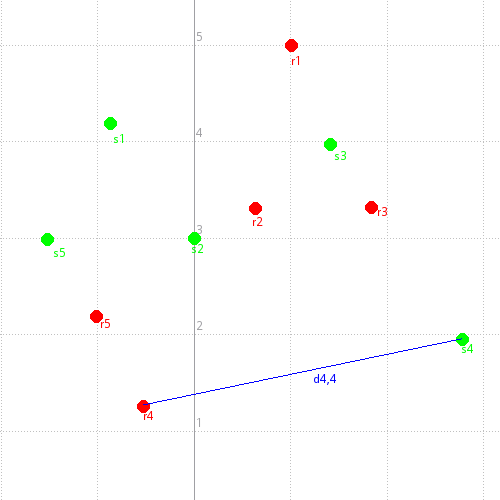
\includegraphics[width=0.5\textwidth]{pictures/model-variables.png}
        \end{wrapfigure}
        Oznaczenia
        \begin{itemize}
            \item $L = \{\lo, \ldots, \ln\}$ - połączenia
            \item $\li = (\si, \ri)$ \\ $\si$ - nadawca i $\ri$ - odbiorca
            \item $\dij = d(\si, \rj)$ \\ odległość pomiędzy nadawcą $\si$ a odbiorcą $\rj$
            \item $\dii$ - długość połączenia $\li$
        \end{itemize}
        Założenia
        \begin{itemize}
            \item Znormalizowane dane \\ $\forall_{\si, \rj} \dij \geq 1$
            \item Każdy nadawca i odbiorca należy do dokładnie jednego połączenia
            \item Jednostkowe obciążenia
        \end{itemize}
    \end{frame}
    \begin{frame}
        \frametitle{Model}
        \begin{wrapfigure}{R}{0.5\textwidth}
            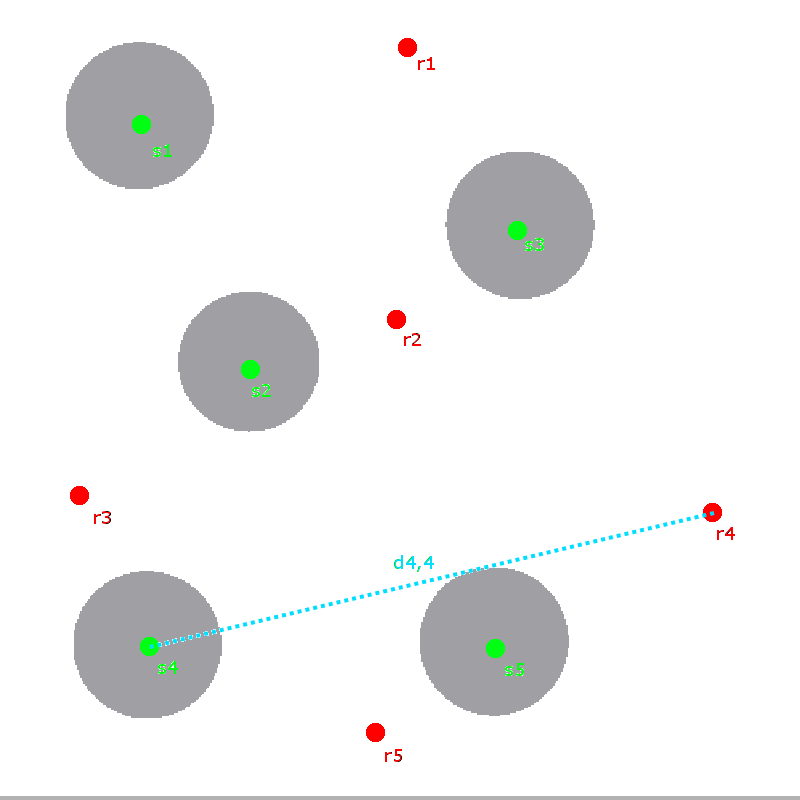
\includegraphics[width=0.5\textwidth]{pictures/model-diagram1.png}
            \caption{$\alpha=2, \beta=1, P=10$}
        \end{wrapfigure}
        Oznaczenia cd.:
        \begin{itemize}
            \item $P(\si)$ - moc nadawcy
            \item $\dij^{-\alpha}$ - współczynnik straty sygnału
            \item $\alpha$ - dobierana doświadczalnie, zależna od warunków otoczenia, zazwyczaj $2 \le \alpha \leq 6$
            \item $P_{\ri}(\si) = P(\si) / \dii^\alpha$ - moc sygnału połączenia $\li$
            \item $I_{\rj}(\si) = P_{\rj}(\si)$ - interferencja wprowadzana przez $\si$ dla odbiorcy $\rj$
        \end{itemize}
    \end{frame}
    \begin{frame}
        \frametitle{Model}
        \begin{wrapfigure}{R}{0.5\textwidth}
            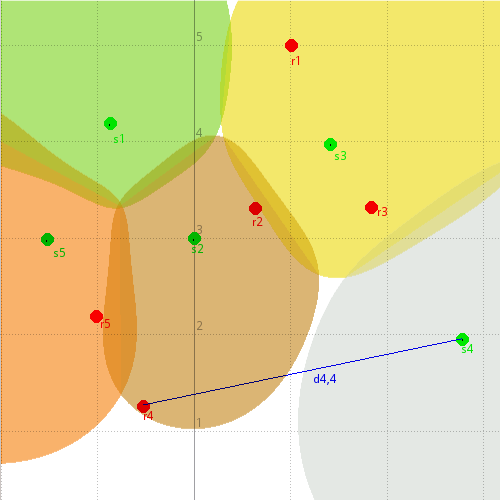
\includegraphics[width=0.5\textwidth]{pictures/model-diagram2.png}
            \caption{$\alpha=2, \beta=1, P=100$}
        \end{wrapfigure}
        Oznaczenia cd.:
        \begin{itemize}
            \item $S_t = {\lo, \ldots, \lm}$ - zbiór połączeń w danym przedziale czasowym
            \item $I_{\ri} = I_{\ri}(S_t) = \sum_{\lj \in S_t, \lj \neq l_i} I_{\ri}(\sj)$ - całkowita interferencja dla odbiorcy $\ri$
            \item $N$ - szum otoczenia
            \item $SINR_{\li} = SINR_{\li}(S_t) = \frac{P_{\ri}(\si)}{I_{\ri} + N}$ - [signal-to-interference-plus-noise-ratio] współczynnik sygnału do interferencji
        \end{itemize}
    \end{frame}
    \begin{frame}
        \frametitle{Model}
        \begin{wrapfigure}{R}{0.5\textwidth}
            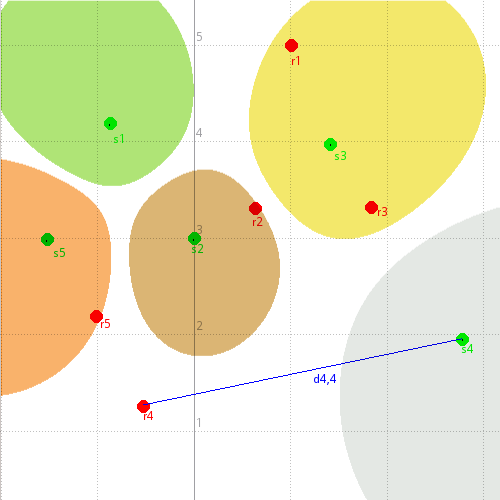
\includegraphics[width=0.5\textwidth]{pictures/model-diagram3.png}
            \caption{$\alpha=2, \beta=1, P=1000$}
        \end{wrapfigure}
        Oznaczenia cd.:
        \begin{itemize}
            \item $\beta$ - współczynnik odbioru sygnału, zależny od sprzętu
            \item sygnał jest poprawnie odbierany wtw. $SINR_{\li} \geq \beta$
            \item harmonogram $S = \{S_1, \ldots, S_T\}$ jest poprawny jeśli $\forall_{S_t \in S} \forall_{\li \in S_t} SINR_{\li}(S_t) \geq \beta$
        \end{itemize}
    \end{frame}
\subsection{Problemy}
    \begin{frame}
        \frametitle{Problemy}
        \begin{wrapfigure}{R}{0.5\textwidth}
            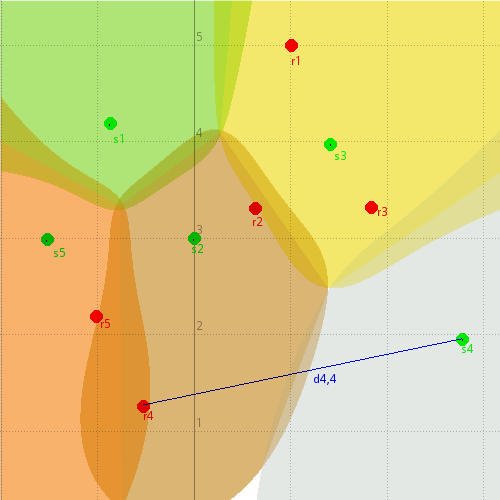
\includegraphics[width=0.5\textwidth]{pictures/model-diagram4.png}
            \caption{$\alpha=2, \beta=1, P=100000$}
        \end{wrapfigure}
        Problemy:
        \begin{itemize}
            \item (Weighted) One-Slot - jak najwięcej nadających na raz
            \item Multi-Slot - jak najmniej przedziałów
            \item Regulacja mocy - każdy może nadawać z różną mocą
        \end{itemize}
    \end{frame}

\section{NP-Trudność}
\subsection{Twierdzenie}
\begin{frame}
    \frametitle{NP-trudność}
    \begin{theorem}
        Problem Multi-Slot w modelu SINR jest NP-trudny.
    \end{theorem}
    \begin{definition}[Problem Podziału]
        Mając dany skończony zbiór liczb całkowitych określić czy istnieje jego podział na dwa rozłączne podzbiory o równej sumie elementów.
    \end{definition}
    \begin{fact}
        Problem Podziału jest NP-zupełny.
    \end{fact}
    \begin{block}{Dowód}
        Pokażemy wielomianową redukcje Problemu Podziału do problemu Multi-Slot w modelu SINR.
    \end{block}
\end{frame}
\subsection{Dowód}
\begin{frame}
    \frametitle{NP-trudność}
    \begin{theorem}
        Problem Multi-Slot w modelu SINR jest NP-trudny.
    \end{theorem}
    \begin{wrapfigure}{R}{0.4\textwidth}
        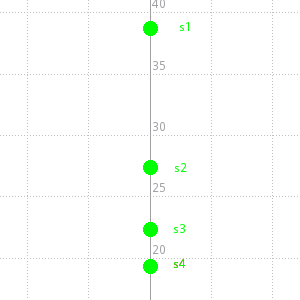
\includegraphics[width=0.4\textwidth]{pictures/np-placement1.png}
    \end{wrapfigure}
    \begin{block}{Dowód(Schemat)}
        \begin{itemize}
            \item $I = \{i_1, \ldots. i_n\}$ - zbiór liczb z Problemu Podziału o sumie $\sigma$
            \item BSO wszystkie elementy $I$ są dodatnie i różne %(?)
            \item $L = \{l_1, \ldots, l_{n+2}\}$ - zbiór połączeń dla Multi-Slota
            \item $\forall_{1 \leq j \leq n} pos(s_j) = (P\cdot{i_j}^\frac{-1}{\alpha}, 0)$ - pozycja nadawców
            \item $d_{min} = P^\frac{1}{\alpha}\cdot\frac{(i_{max}-1)^\frac{-1}{\alpha}-(i_{max})^\frac{-1}{\alpha}}{1+(n\beta)^\frac{1}{\alpha}}$
            \item $\forall_{1 \leq j \leq n} pos(r_j) = pos(s_j) + (d_{min}, 0)$ - pozycja odbiorców
        \end{itemize}
    \end{block}
\end{frame}
\begin{frame}
    \frametitle{NP-trudność}
    \begin{theorem}
        Problem Multi-Slot w modelu SINR jest NP-trudny.
    \end{theorem}
    \begin{wrapfigure}{R}{0.4\textwidth}
        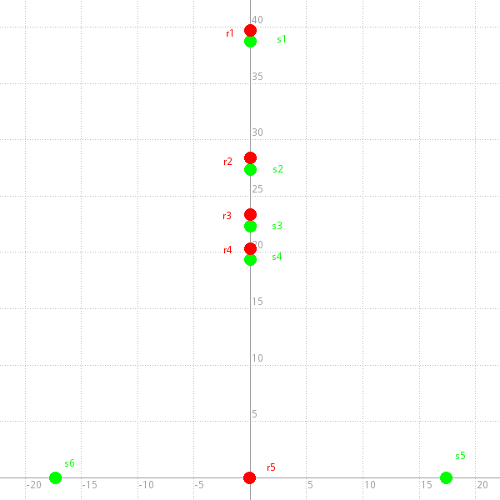
\includegraphics[width=0.4\textwidth]{pictures/np-placement2.png}
    \end{wrapfigure}
    \begin{block}{Dowód(Schemat cd.)}
        \begin{itemize}
            \item $pos(r_{n+1}) = pos(r_{n+2}) = (0, 0)$
            \item $pos(s_{n+1}) = (0, 2P\cdot(\beta\sigma)^{\frac{-1}{\alpha}})$
            \item $pos(s_{n+2}) = (0, -2P\cdot(\beta\sigma)^{\frac{-1}{\alpha}})$
            \item W jednym przedziale się nie da ($r_{n+1}$ oraz $r_{n+2}$ są w tym samym miejscu)
            \item Da się w dwóch wtw. mamy rozwiązanie Problemu Podziału
        \end{itemize}
    \end{block}
\end{frame}
\begin{frame}
    \frametitle{NP-trudność}
    \begin{theorem}
        Problem Multi-Slot w modelu SINR jest NP-trudny.
    \end{theorem}
    \begin{wrapfigure}{R}{0.4\textwidth}
        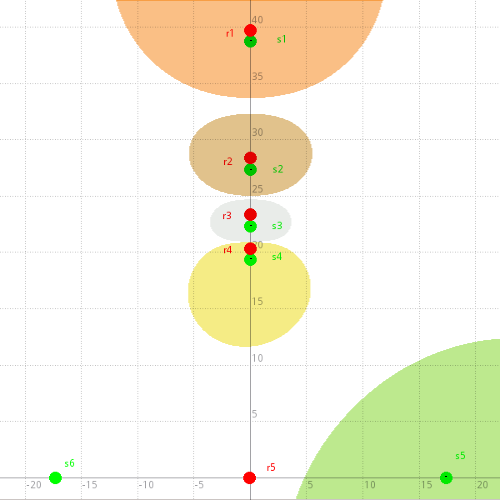
\includegraphics[width=0.4\textwidth]{pictures/np-placement3.png}
    \end{wrapfigure}
    \begin{block}{Dowód(Schemat cd.)}
        \begin{lemma}
            Niech $L_i = \{l_j: 1 \leq j \leq n + 1, i \neq j\}$.\\
            Dla każdego $i \leq n$ kiedy $l_i$ jest zaplanowany wraz z elementami $L_i$ wartość $SINR \ge \beta$.
        \end{lemma}
        \begin{itemize}
            \item $P_{r_{n+1}}(s_{n+1}) = \frac{\beta\sigma}{2}$
            \item $I_{r_{n+1}}(s_j) = i_j$
            \item $I_{r_{n+1}} = \frac{\sigma}{2}$
            \item $SINR_{r_{n+1}} \geq \beta$
        \end{itemize}
    \end{block}
\end{frame}

\section{Approx}
\section{Wypukłości itd.}
\section{TODO}
\end{document}
